\section{Night-, twilight- and day-sky model}
\label{sec:sky}

For faint targets the sky, not the detector, is the adversary: once the
background electrons in the aperture outnumber the source electrons, the
S/N grows only as the square root of exposure time and every magnitude of
extra sky brightness costs a factor 2.5 in required time. An ETC is
therefore only as honest as its sky model. \spetc{}'s model has an
unusual property for a tool in this class: it is \emph{position- and
time-dependent}. The same target yields a different sky --- and a
different exposure recommendation --- depending on where it sits with
respect to the ecliptic (zodiacal light), the Milky Way (integrated
starlight), the Moon (scattered moonlight), the Sun (twilight), and the
local zenith (airglow path length), all evaluated per time sample of the
night. The components and their assembly are as follows.

\subsection{Dark sky}

Surface brightnesses are budgeted in \emph{S10 units} — the brightness
equivalent to one star of visual magnitude 10 per square degree, a linear
(flux-like) unit in which components simply add; the conversion to
magnitudes per square arcsecond is $\mu = 27.78 - 2.5\log_{10}q$ for a
brightness of $q$ S10. The dark-sky normalization is the broad-band
$U$--$K$ surface-brightness table of Table~\ref{tab:sky} (from the ING
model of \citealt{bennellison1998}), corrected for the pointing and epoch
through the S10 component budget
\begin{equation}
  q_3 \;=\; q_{\rm air}\,V(z)\,\mathcal{E}(z) \;+\;
            q_{\rm zod}(|\beta|)\,g(\epsilon) \;+\; q_\ast(|b|),
\end{equation}
normalized to the dark reference composition $q_{\rm ref} = 145 + 60$ S10.
The components are:
\begin{itemize}
\item \textbf{Airglow}: $q_{\rm air} = 145 + 130\,(a-0.8)/1.2$ S10, where the
  solar-cycle activity $a \in [0.8, 2.0]$ is interpolated between the
  tabulated solar minima (airglow is excited by solar UV, so it roughly
  doubles from solar minimum to maximum). The line-of-sight enhancement is
  the van Rhijn path-length law \citep{vanrhijn1921} for an emitting layer
  at height $\hat h = \SI{90}{km}$,
  \begin{equation}
    V(z) = \Big[1 - \Big(\tfrac{R_\oplus}{R_\oplus+\hat h}\sin z\Big)^2\Big]^{-1/2},
    \label{eq:vanrhijn}
  \end{equation}
  which is sub-linear in airmass and bounded ($V \simeq 6$) at the horizon
  (Fig.~\ref{fig:skypos}, right). The raw van Rhijn factor is however
  never observed: the emitted light must still descend through the
  troposphere along the same slant, which attenuates it by
  \begin{equation}
    \mathcal{E}(z) \;=\; 10^{-0.4\,k_V\,[X_{\rm KY}(z) - 1]},
  \end{equation}
  with $k_V$ the $V$ extinction coefficient and $X_{\rm KY}$ the
  \citet{kasten1989} line-of-sight airmass
  $[\cos z + 0.50572\,(96.07995-z)^{-1.6364}]^{-1}$, finite
  ($X \simeq 38$) at the horizon. Near the horizon $\mathcal{E}$
  partially cancels the van Rhijn enhancement, matching the observed
  behaviour (v10.2).
\item \textbf{Zodiacal light} — sunlight scattered by interplanetary
  dust: $q_{\rm zod} = 140 - 90 \sin|\beta|$ S10 for
  $|\beta| < 60^\circ$, else 60 S10, symmetric about the ecliptic. This
  latitude law describes the anti-solar sky; towards the Sun the dust
  column and the scattering efficiency both rise steeply. The solar
  elongation $\epsilon$ (the field's angular distance from the Sun)
  therefore multiplies it by the factor
  \begin{equation}
    g(\epsilon) \;=\;
    \begin{cases}
      (\epsilon/110^\circ)^{-2.3} & 30^\circ \le \epsilon < 110^\circ\\
      1 & \epsilon \ge 110^\circ,
    \end{cases}
  \end{equation}
  a power-law fit to the \citet{leinert1998} tables at $\beta = 0$
  ($\sim$4$\times$ brighter at $\epsilon = 60^\circ$); below $30^\circ$
  the line of sight is unobservable and the factor is held (v10.2).
\item \textbf{Integrated starlight} — the summed light of unresolved
  stars: $q_\ast = 100\,e^{-|b|/10^\circ}$ S10, falling away from the
  galactic plane.
\end{itemize}
The field's ecliptic and galactic latitudes are computed from the entered
ICRS coordinates with \code{astropy}; the sky is therefore genuinely
position-dependent (Fig.~\ref{fig:skypos}, left).

\begin{table}
\centering
\caption{Built-in broad-band sky data ($U$--$K$): dark-sky surface
brightness, extinction coefficient, Vega zero point and
Krisciunas--Schaefer lunar colour factor.}
\label{tab:sky}
\begin{tabular}{lccccc}
\toprule
Band & $\lambda$ [\si{\angstrom}] & $\mu_{\rm dark}$ [mag/$''^2$] &
$k$ [mag/X] & $Z_\nu^{\rm Vega}$ [Jy] & lunar factor \\
\midrule
$U$ &  3650 & 22.0 & 0.550 & 1810 &  2.00 \\
$B$ &  4450 & 22.7 & 0.250 & 4260 &  1.60 \\
$V$ &  5510 & 21.9 & 0.150 & 3640 &  2.40 \\
$R$ &  6580 & 21.0 & 0.090 & 3080 &  3.00 \\
$I$ &  8060 & 20.0 & 0.060 & 2550 &  5.90 \\
$Z$ & 10000 & 18.8 & 0.050 & 2250 &  8.94 \\
$J$ & 12500 & 16.1 & 0.100 & 1594 & 13.06 \\
$H$ & 16500 & 14.7 & 0.110 & 1024 & 18.09 \\
$K$ & 22000 & 12.5 & 0.070 &  667 & 24.04 \\
\bottomrule
\end{tabular}
\end{table}

\begin{figure}
  \centering
  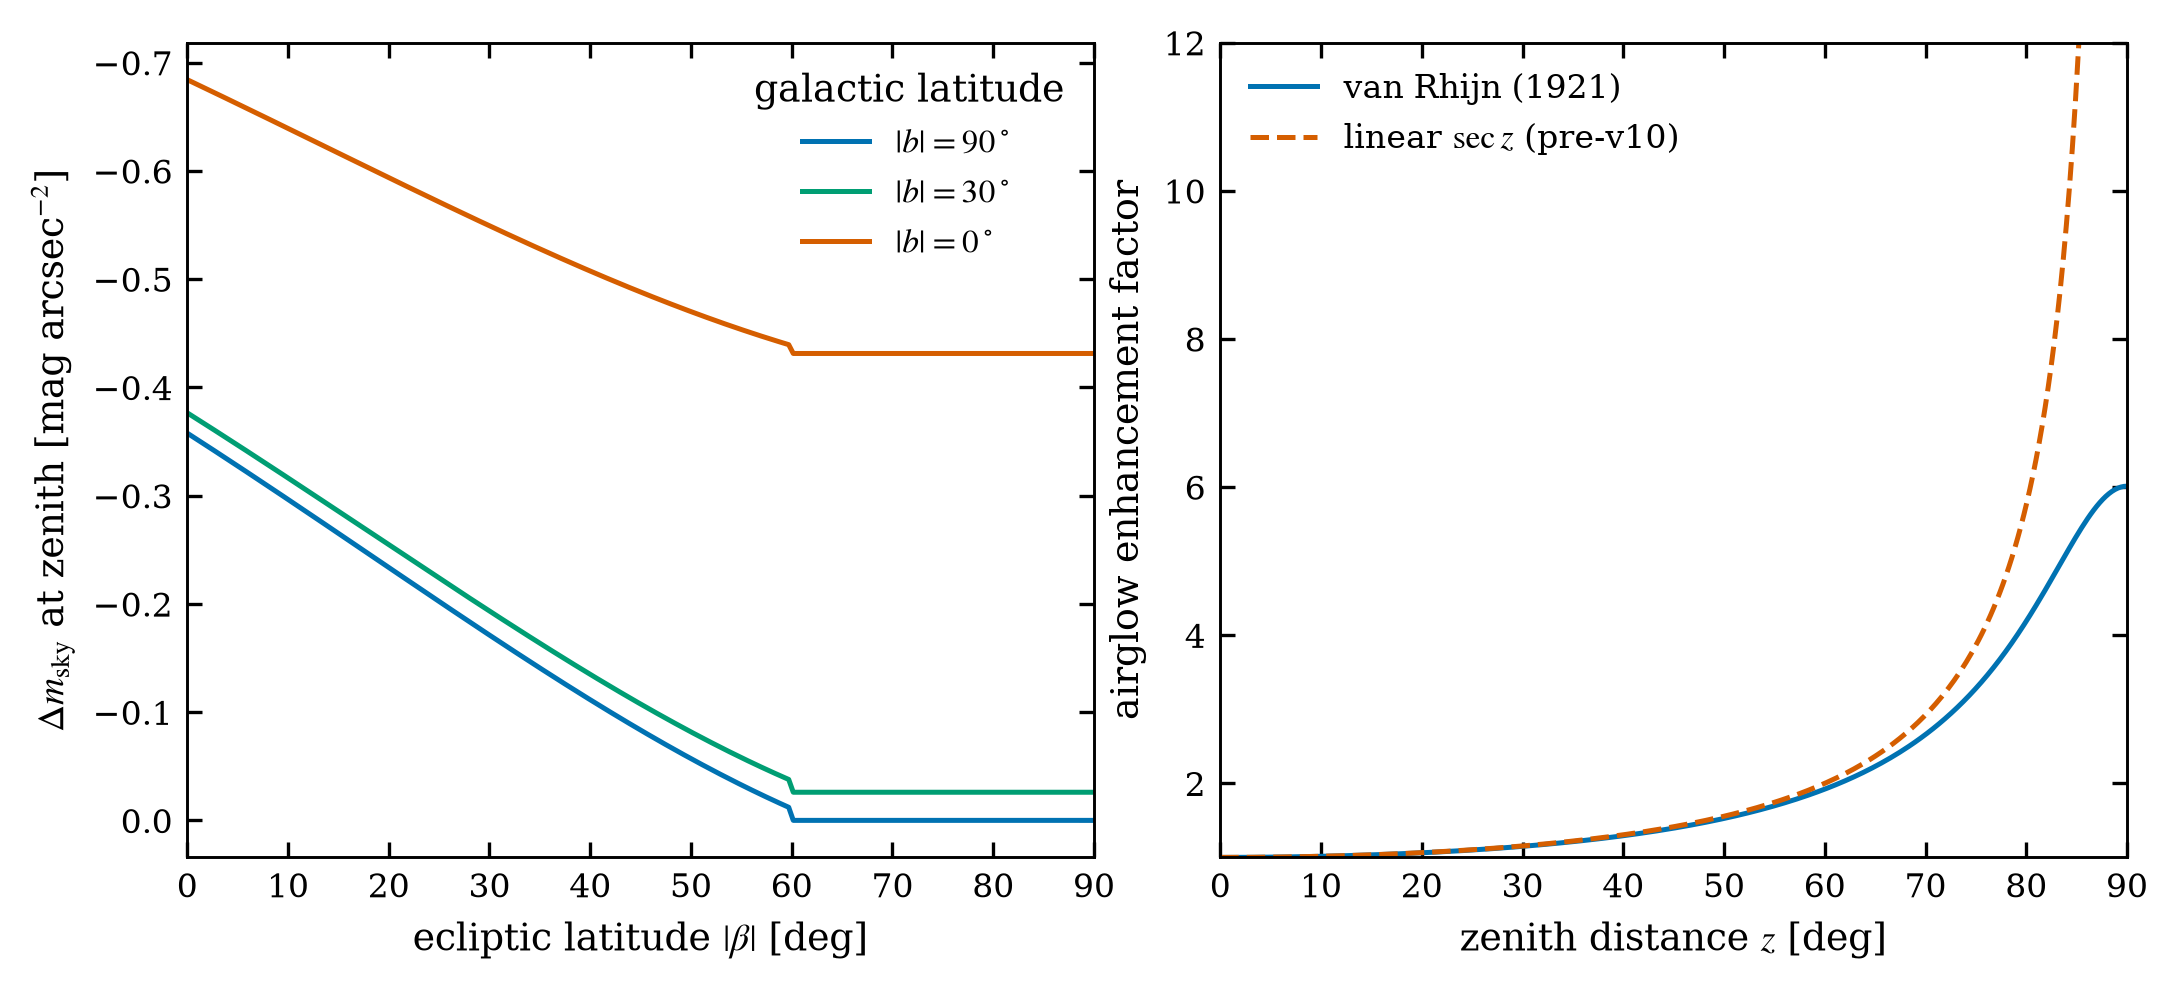
\includegraphics[width=\textwidth]{figures/fig_04_sky_position.png}
  \caption{Left: zenith dark-sky brightening relative to the tabulated
  values as a function of ecliptic latitude, for three galactic latitudes
  (solar minimum). Right: van Rhijn airglow enhancement versus the linear
  $\sec z$ scaling used before v10.}
  \label{fig:skypos}
\end{figure}

\subsection{Moonlight}

Moonlight follows \citet{krisciunas1991}. The lunar phase angle $\alpha$
is the Sun--Moon--Earth angle ($0^\circ$ = full Moon, $90^\circ$ =
quarter), computed as $180^\circ$ minus the Sun--Moon elongation. The
lunar illuminance — the flux of moonlight arriving at the top of the
atmosphere — is
$I^\ast = 10^{-0.4(3.84 + 0.026|\alpha| + 4\times10^{-9}\alpha^4)}
\,(\bar d/d_{\rm moon})^2$: the polynomial is K\&S's fit to the lunar
phase curve, and the second factor is the inverse-square modulation by
the topocentric Moon distance $d_{\rm moon}$ around its mean
$\bar d = 384\,400$ km — a $\pm 15\%$ brightness swing over the
anomalistic month that the track supplies per time sample (v10.2). The
scattering function at Moon--target separation $\rho$ is
\begin{equation}
  f(\rho) \;=\; 10^{5.36}\big(1.06 + \cos^2\rho\big) \;+\;
                 10^{6.15 - \rho/40^\circ}.
  \label{eq:ks}
\end{equation}
The scattering function has two physically distinct terms:
$10^{5.36}(1.06+\cos^2\rho)$ is the Rayleigh contribution (molecular
scattering, with its characteristic $1+\cos^2$ angular pattern), and
$10^{6.15-\rho/40^\circ}$ is the aerosol \emph{aureole}, the forward-scattering
halo around the Moon. The moonlit surface brightness in nanoLambert (a
luminance unit; 1 nL converts to 3.8 S10) is
$B_{\rm moon} = I^\ast f(\rho)\,
10^{-0.4kX_{\rm m}}\big(1 - 10^{-0.4kX}\big)$, where $X_{\rm m}$ is the
Moon's airmass (the moonlight is first extinguished on its way down) and
the bracket is the fraction of light scattered \emph{out of} the direct
beam along the target's path — the scattered moonlight the target line of
sight picks up. This is converted to S10 and
distributed over the nine bands with the lunar colour factors of
Table~\ref{tab:sky}. Equation~(\ref{eq:ks}) corrects a long-standing
transcription error in which the constant $10^{5.36}$ appeared inside the
exponent; the two forms diverge by more than three orders of magnitude
within $30^\circ$ of the Moon (Fig.~\ref{fig:ks}).

\begin{figure}
  \centering
  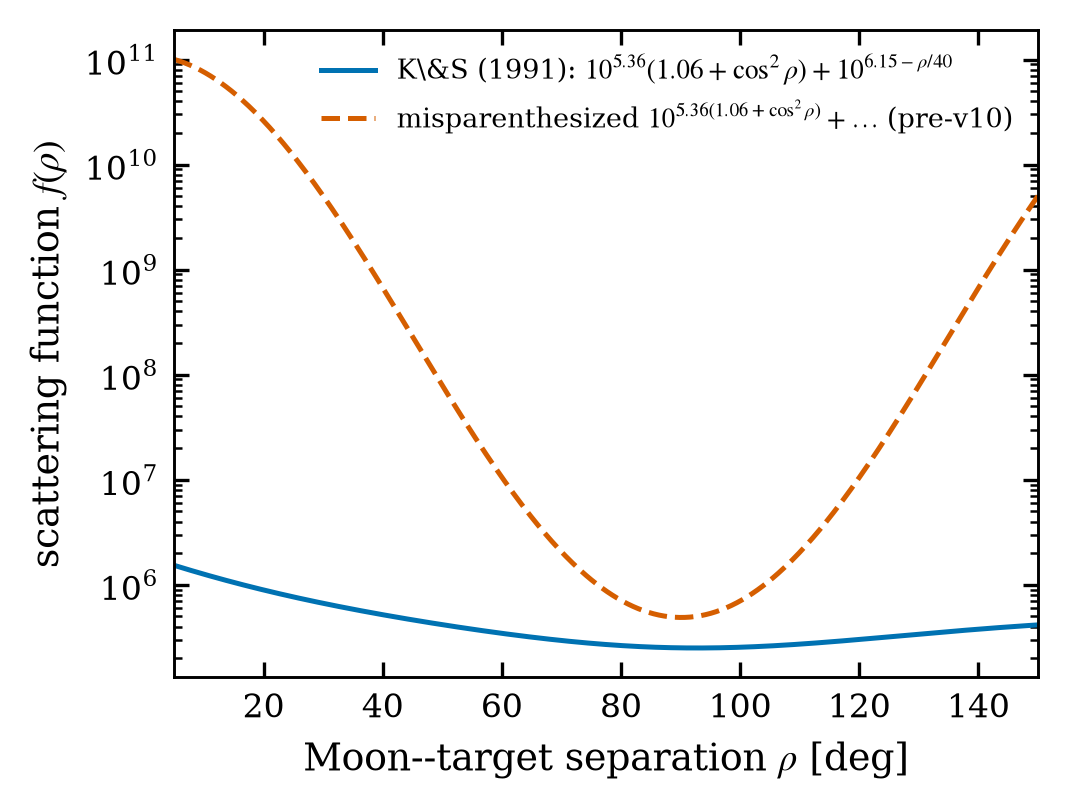
\includegraphics[width=0.62\textwidth]{figures/fig_01_moon_scattering.png}
  \caption{The \citet{krisciunas1991} scattering function (solid) and the
  misparenthesized variant present before v10 (dashed).}
  \label{fig:ks}
\end{figure}

\subsection{SQM and Bortle input}
\label{sec:sqm}

Amateur observers know their sky as a Sky Quality Meter reading (zenith
$V$ surface brightness) or a \citet{bortle2001} class rather than as a
per-band table. In \code{sqm} mode the entered zenith SQM value $\mu_{\rm
SQM}$ replaces the dark-sky normalization directly:
\begin{equation}
  \mu(\lambda_{\rm piv}) \;=\; \mu_{\rm SQM} \;+\;
  \big[\mu_{\rm tab}(\lambda_{\rm piv}) - \mu_{\rm tab}(V)\big],
\end{equation}
i.e.\ the built-in table supplies only the band colour, while the SQM
reading — which already contains the site's light pollution and current
airglow — sets the level. The Krisciunas--Schaefer Moon contribution of
the previous subsection is applied on top unchanged. A Bortle-class
selector fills typical zenith SQM values (21.9, 21.8, 21.6, 21.1, 20.5,
19.8, 19.0, 18.0, 17.0 mag\,arcsec$^{-2}$ for classes 1--9).

\subsection{Twilight and daylight}
\label{sec:daylight}

Between \emph{geometric} Sun altitudes of $-18^\circ$ (end of
astronomical twilight) and $0^\circ$ the dark and daylight skies are
blended linearly in flux — magnitudes cannot be averaged, fluxes can.
Above the horizon a daylight table in the \citet{weaver1947} lineage
supplies the $V$-band surface brightness as a function of solar and sky
zenith distance, mapped to other bands with the dark-sky colours of
Table~\ref{tab:sky}.

The v10.1 physics audit found the daylight table, read directly as
mag/arcsec$^2$, to be $\sim$4.5 magnitudes too \emph{faint}: its values
(8.5--9.2) would make the daytime sky only $\sim$200$\times$ brighter
than a dark night, whereas the physical clear daytime zenith sky is
$\sim$3000--8000 cd/m$^2$, i.e.\ $V \simeq 3.5$--4.5 mag/arcsec$^2$
against the night-sky anchor (21.9 mag/arcsec$^2 \approx
2\times10^{-4}$ cd/m$^2$) — a $\sim$$10^7$ flux ratio. The v10.2 model
therefore keeps the table's \emph{shape} in solar and sky zenith
distance but re-anchors its brightest entry to the physical
$V = 4.0$ mag/arcsec$^2$; the twilight blend inherits the corrected
anchor. Both regimes remain broad-band approximations, clearly flagged
in the user interface, and the original supplied table is preserved in
the source for the day the exact Weaver unit conversion is re-derived.
